% Created by tikzDevice version 0.12.6 on 2025-05-24 13:23:59
% !TEX encoding = UTF-8 Unicode
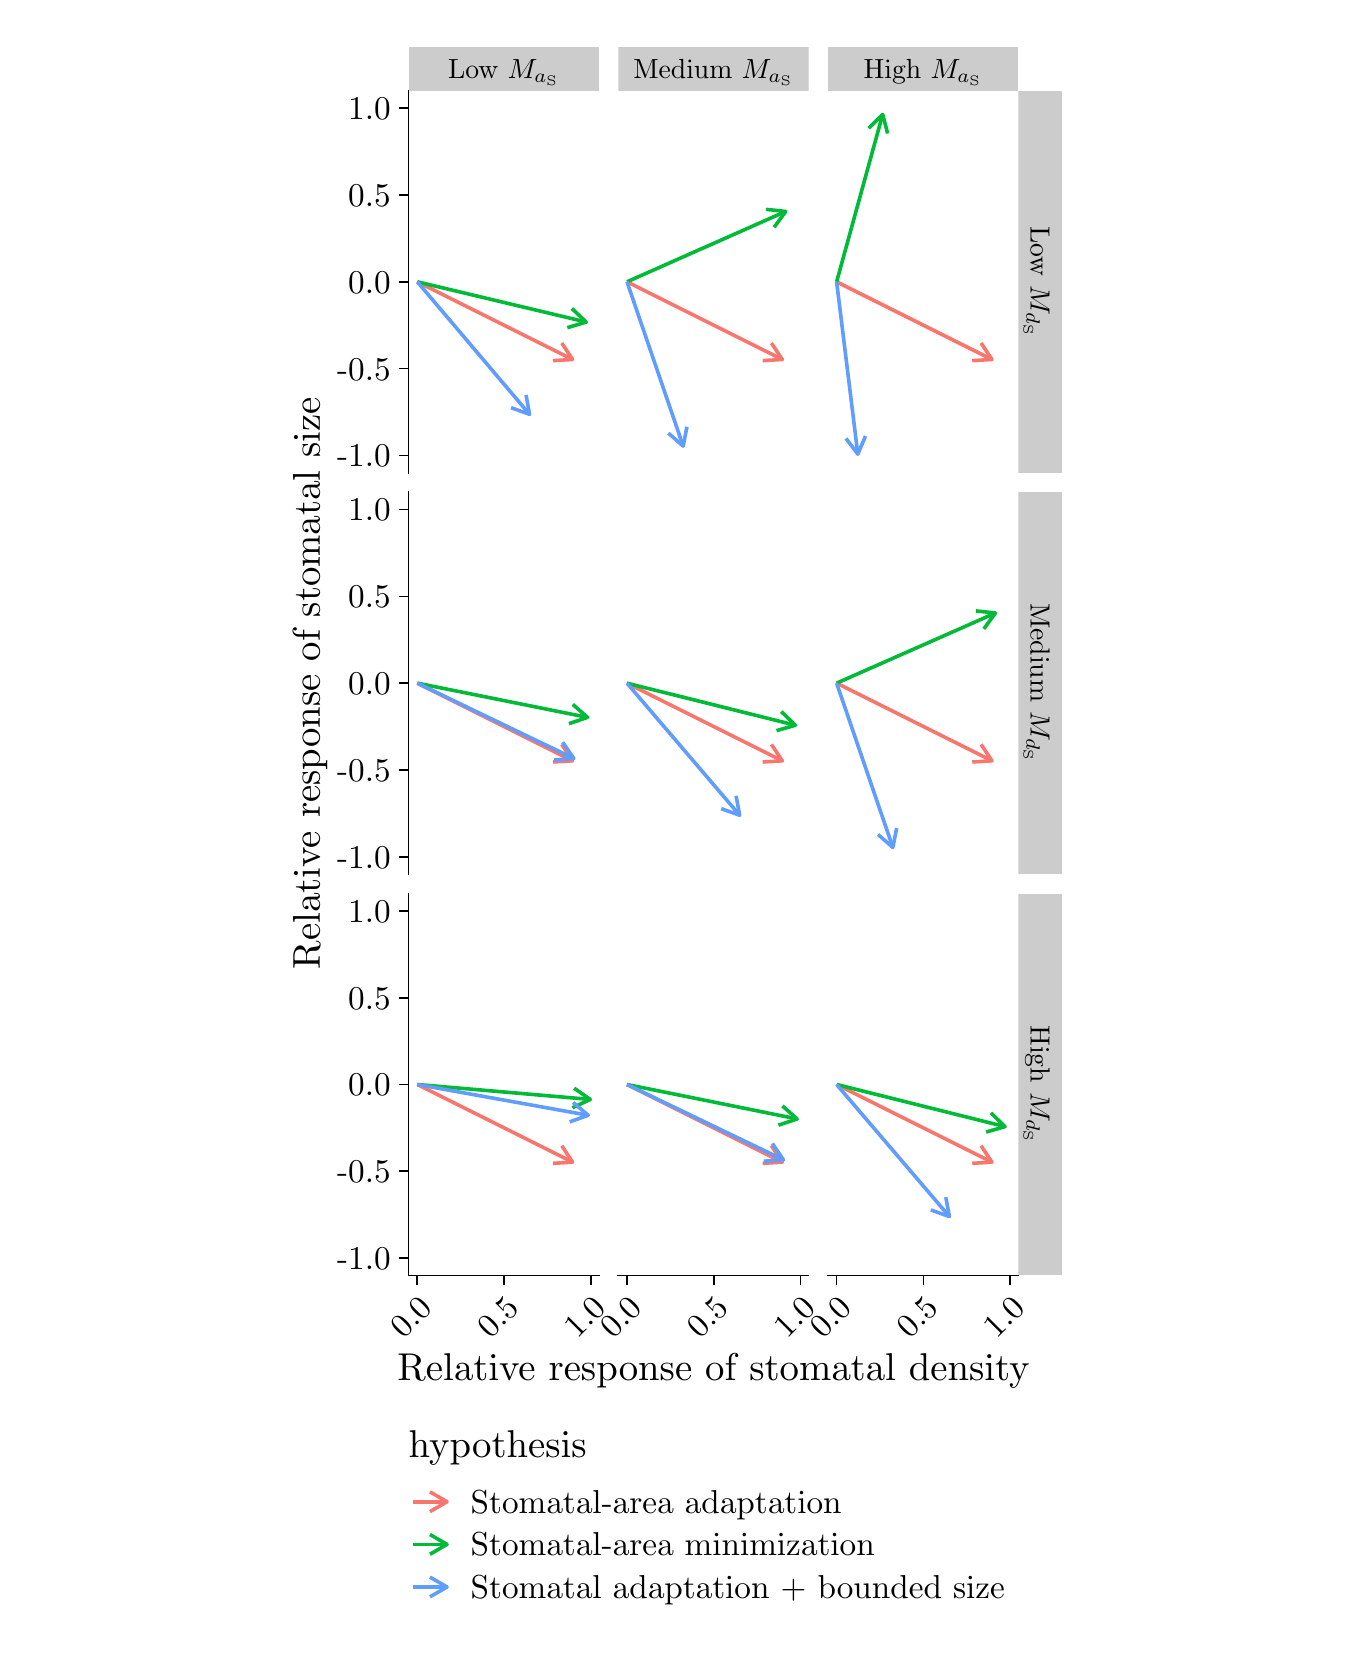
\begin{tikzpicture}[x=1pt,y=1pt]
\definecolor{fillColor}{RGB}{255,255,255}
\path[use as bounding box,fill=fillColor,fill opacity=0.00] (0,0) rectangle (469.75,578.16);
\begin{scope}
\path[clip] (137.67,417.31) rectangle (206.43,555.33);
\definecolor{drawColor}{RGB}{248,118,109}

\path[draw=drawColor,line width= 1.3pt,line join=round] (140.80,486.32) -- (196.91,458.26);

\path[draw=drawColor,line width= 1.3pt,line join=round] (189.81,457.83) --
	(196.91,458.26) --
	(192.99,464.20);
\definecolor{drawColor}{RGB}{0,186,56}

\path[draw=drawColor,line width= 1.3pt,line join=round] (140.80,486.32) -- (201.83,471.78);

\path[draw=drawColor,line width= 1.3pt,line join=round] (195.01,469.75) --
	(201.83,471.78) --
	(196.66,476.67);
\definecolor{drawColor}{RGB}{97,156,255}

\path[draw=drawColor,line width= 1.3pt,line join=round] (140.80,486.32) -- (181.35,438.44);

\path[draw=drawColor,line width= 1.3pt,line join=round] (174.65,440.85) --
	(181.35,438.44) --
	(180.08,445.44);
\end{scope}
\begin{scope}
\path[clip] (137.67,272.28) rectangle (206.43,410.31);
\definecolor{drawColor}{RGB}{248,118,109}

\path[draw=drawColor,line width= 1.3pt,line join=round] (140.80,341.29) -- (196.91,313.24);

\path[draw=drawColor,line width= 1.3pt,line join=round] (189.81,312.81) --
	(196.91,313.24) --
	(192.99,319.17);
\definecolor{drawColor}{RGB}{0,186,56}

\path[draw=drawColor,line width= 1.3pt,line join=round] (140.80,341.29) -- (202.31,328.93);

\path[draw=drawColor,line width= 1.3pt,line join=round] (195.57,326.65) --
	(202.31,328.93) --
	(196.97,333.63);
\definecolor{drawColor}{RGB}{97,156,255}

\path[draw=drawColor,line width= 1.3pt,line join=round] (140.80,341.29) -- (197.33,314.08);

\path[draw=drawColor,line width= 1.3pt,line join=round] (190.24,313.55) --
	(197.33,314.08) --
	(193.32,319.96);
\end{scope}
\begin{scope}
\path[clip] (137.67,127.26) rectangle (206.43,265.28);
\definecolor{drawColor}{RGB}{248,118,109}

\path[draw=drawColor,line width= 1.3pt,line join=round] (140.80,196.27) -- (196.91,168.21);

\path[draw=drawColor,line width= 1.3pt,line join=round] (189.81,167.79) --
	(196.91,168.21) --
	(192.99,174.15);
\definecolor{drawColor}{RGB}{0,186,56}

\path[draw=drawColor,line width= 1.3pt,line join=round] (140.80,196.27) -- (203.30,190.87);

\path[draw=drawColor,line width= 1.3pt,line join=round] (196.86,187.86) --
	(203.30,190.87) --
	(197.47,194.95);
\definecolor{drawColor}{RGB}{97,156,255}

\path[draw=drawColor,line width= 1.3pt,line join=round] (140.80,196.27) -- (202.55,185.16);

\path[draw=drawColor,line width= 1.3pt,line join=round] (195.85,182.75) --
	(202.55,185.16) --
	(197.11,189.75);
\end{scope}
\begin{scope}
\path[clip] (213.43,417.31) rectangle (282.19,555.33);
\definecolor{drawColor}{RGB}{248,118,109}

\path[draw=drawColor,line width= 1.3pt,line join=round] (216.56,486.32) -- (272.67,458.26);

\path[draw=drawColor,line width= 1.3pt,line join=round] (265.57,457.83) --
	(272.67,458.26) --
	(268.75,464.20);
\definecolor{drawColor}{RGB}{0,186,56}

\path[draw=drawColor,line width= 1.3pt,line join=round] (216.56,486.32) -- (273.91,511.75);

\path[draw=drawColor,line width= 1.3pt,line join=round] (269.72,506.00) --
	(273.91,511.75) --
	(266.84,512.50);
\definecolor{drawColor}{RGB}{97,156,255}

\path[draw=drawColor,line width= 1.3pt,line join=round] (216.56,486.32) -- (236.86,426.96);

\path[draw=drawColor,line width= 1.3pt,line join=round] (231.50,431.63) --
	(236.86,426.96) --
	(238.23,433.94);
\end{scope}
\begin{scope}
\path[clip] (213.43,272.28) rectangle (282.19,410.31);
\definecolor{drawColor}{RGB}{248,118,109}

\path[draw=drawColor,line width= 1.3pt,line join=round] (216.56,341.29) -- (272.67,313.24);

\path[draw=drawColor,line width= 1.3pt,line join=round] (265.57,312.81) --
	(272.67,313.24) --
	(268.75,319.17);
\definecolor{drawColor}{RGB}{0,186,56}

\path[draw=drawColor,line width= 1.3pt,line join=round] (216.56,341.29) -- (277.42,326.09);

\path[draw=drawColor,line width= 1.3pt,line join=round] (270.58,324.13) --
	(277.42,326.09) --
	(272.31,331.03);
\definecolor{drawColor}{RGB}{97,156,255}

\path[draw=drawColor,line width= 1.3pt,line join=round] (216.56,341.29) -- (257.28,293.57);

\path[draw=drawColor,line width= 1.3pt,line join=round] (250.58,295.95) --
	(257.28,293.57) --
	(255.99,300.57);
\end{scope}
\begin{scope}
\path[clip] (213.43,127.26) rectangle (282.19,265.28);
\definecolor{drawColor}{RGB}{248,118,109}

\path[draw=drawColor,line width= 1.3pt,line join=round] (216.56,196.27) -- (272.67,168.21);

\path[draw=drawColor,line width= 1.3pt,line join=round] (265.57,167.79) --
	(272.67,168.21) --
	(268.75,174.15);
\definecolor{drawColor}{RGB}{0,186,56}

\path[draw=drawColor,line width= 1.3pt,line join=round] (216.56,196.27) -- (278.05,183.83);

\path[draw=drawColor,line width= 1.3pt,line join=round] (271.30,181.57) --
	(278.05,183.83) --
	(272.72,188.54);
\definecolor{drawColor}{RGB}{97,156,255}

\path[draw=drawColor,line width= 1.3pt,line join=round] (216.56,196.27) -- (273.09,169.07);

\path[draw=drawColor,line width= 1.3pt,line join=round] (266.00,168.54) --
	(273.09,169.07) --
	(269.08,174.95);
\end{scope}
\begin{scope}
\path[clip] (289.19,417.31) rectangle (357.94,555.33);
\definecolor{drawColor}{RGB}{248,118,109}

\path[draw=drawColor,line width= 1.3pt,line join=round] (292.31,486.32) -- (348.43,458.26);

\path[draw=drawColor,line width= 1.3pt,line join=round] (341.32,457.83) --
	(348.43,458.26) --
	(344.51,464.20);
\definecolor{drawColor}{RGB}{0,186,56}

\path[draw=drawColor,line width= 1.3pt,line join=round] (292.31,486.32) -- (308.95,546.81);

\path[draw=drawColor,line width= 1.3pt,line join=round] (310.75,539.92) --
	(308.95,546.81) --
	(303.89,541.81);
\definecolor{drawColor}{RGB}{97,156,255}

\path[draw=drawColor,line width= 1.3pt,line join=round] (292.31,486.32) -- (299.97,424.05);

\path[draw=drawColor,line width= 1.3pt,line join=round] (295.69,429.73) --
	(299.97,424.05) --
	(302.75,430.60);
\end{scope}
\begin{scope}
\path[clip] (289.19,272.28) rectangle (357.94,410.31);
\definecolor{drawColor}{RGB}{248,118,109}

\path[draw=drawColor,line width= 1.3pt,line join=round] (292.31,341.29) -- (348.43,313.24);

\path[draw=drawColor,line width= 1.3pt,line join=round] (341.32,312.81) --
	(348.43,313.24) --
	(344.51,319.17);
\definecolor{drawColor}{RGB}{0,186,56}

\path[draw=drawColor,line width= 1.3pt,line join=round] (292.31,341.29) -- (349.70,366.64);

\path[draw=drawColor,line width= 1.3pt,line join=round] (345.50,360.90) --
	(349.70,366.64) --
	(342.63,367.40);
\definecolor{drawColor}{RGB}{97,156,255}

\path[draw=drawColor,line width= 1.3pt,line join=round] (292.31,341.29) -- (312.63,281.94);

\path[draw=drawColor,line width= 1.3pt,line join=round] (307.27,286.61) --
	(312.63,281.94) --
	(314.00,288.92);
\end{scope}
\begin{scope}
\path[clip] (289.19,127.26) rectangle (357.94,265.28);
\definecolor{drawColor}{RGB}{248,118,109}

\path[draw=drawColor,line width= 1.3pt,line join=round] (292.31,196.27) -- (348.43,168.21);

\path[draw=drawColor,line width= 1.3pt,line join=round] (341.32,167.79) --
	(348.43,168.21) --
	(344.51,174.15);
\definecolor{drawColor}{RGB}{0,186,56}

\path[draw=drawColor,line width= 1.3pt,line join=round] (292.31,196.27) -- (353.18,181.05);

\path[draw=drawColor,line width= 1.3pt,line join=round] (346.34,179.10) --
	(353.18,181.05) --
	(348.06,186.00);
\definecolor{drawColor}{RGB}{97,156,255}

\path[draw=drawColor,line width= 1.3pt,line join=round] (292.31,196.27) -- (333.06,148.57);

\path[draw=drawColor,line width= 1.3pt,line join=round] (326.35,150.94) --
	(333.06,148.57) --
	(331.76,155.56);
\end{scope}
\begin{scope}
\path[clip] (137.67,555.33) rectangle (206.43,571.16);
\definecolor{fillColor}{gray}{0.80}

\path[fill=fillColor] (137.67,555.33) rectangle (206.43,571.16);
\definecolor{drawColor}{RGB}{0,0,0}

\node[text=drawColor,anchor=base,inner sep=0pt, outer sep=0pt, scale=  1.00] at (172.05,559.80) {Low $M_{a_\mathrm{S}}$};
\end{scope}
\begin{scope}
\path[clip] (213.43,555.33) rectangle (282.19,571.16);
\definecolor{fillColor}{gray}{0.80}

\path[fill=fillColor] (213.43,555.33) rectangle (282.19,571.16);
\definecolor{drawColor}{RGB}{0,0,0}

\node[text=drawColor,anchor=base,inner sep=0pt, outer sep=0pt, scale=  1.00] at (247.81,559.80) {Medium $M_{a_\mathrm{S}}$};
\end{scope}
\begin{scope}
\path[clip] (289.19,555.33) rectangle (357.94,571.16);
\definecolor{fillColor}{gray}{0.80}

\path[fill=fillColor] (289.19,555.33) rectangle (357.94,571.16);
\definecolor{drawColor}{RGB}{0,0,0}

\node[text=drawColor,anchor=base,inner sep=0pt, outer sep=0pt, scale=  1.00] at (323.56,559.80) {High $M_{a_\mathrm{S}}$};
\end{scope}
\begin{scope}
\path[clip] (357.94,417.31) rectangle (373.77,555.33);
\definecolor{fillColor}{gray}{0.80}

\path[fill=fillColor] (357.94,417.31) rectangle (373.77,555.33);
\definecolor{drawColor}{RGB}{0,0,0}

\node[text=drawColor,rotate=-90.00,anchor=base,inner sep=0pt, outer sep=0pt, scale=  1.00] at (362.41,486.32) {Low $M_{d_\mathrm{S}}$};
\end{scope}
\begin{scope}
\path[clip] (357.94,272.28) rectangle (373.77,410.31);
\definecolor{fillColor}{gray}{0.80}

\path[fill=fillColor] (357.94,272.28) rectangle (373.77,410.31);
\definecolor{drawColor}{RGB}{0,0,0}

\node[text=drawColor,rotate=-90.00,anchor=base,inner sep=0pt, outer sep=0pt, scale=  1.00] at (362.41,341.29) {Medium $M_{d_\mathrm{S}}$};
\end{scope}
\begin{scope}
\path[clip] (357.94,127.26) rectangle (373.77,265.28);
\definecolor{fillColor}{gray}{0.80}

\path[fill=fillColor] (357.94,127.26) rectangle (373.77,265.28);
\definecolor{drawColor}{RGB}{0,0,0}

\node[text=drawColor,rotate=-90.00,anchor=base,inner sep=0pt, outer sep=0pt, scale=  1.00] at (362.41,196.27) {High $M_{d_\mathrm{S}}$};
\end{scope}
\begin{scope}
\path[clip] (  0.00,  0.00) rectangle (469.75,578.16);
\definecolor{drawColor}{RGB}{0,0,0}

\path[draw=drawColor,line width= 0.6pt,line join=round,line cap=rect] (137.67,127.26) --
	(206.43,127.26);
\end{scope}
\begin{scope}
\path[clip] (  0.00,  0.00) rectangle (469.75,578.16);
\definecolor{drawColor}{RGB}{0,0,0}

\path[draw=drawColor,line width= 0.6pt,line join=round] (140.80,123.76) --
	(140.80,127.26);

\path[draw=drawColor,line width= 0.6pt,line join=round] (172.17,123.76) --
	(172.17,127.26);

\path[draw=drawColor,line width= 0.6pt,line join=round] (203.54,123.76) --
	(203.54,127.26);
\end{scope}
\begin{scope}
\path[clip] (  0.00,  0.00) rectangle (469.75,578.16);
\definecolor{drawColor}{RGB}{0,0,0}

\node[text=drawColor,rotate= 45.00,anchor=base east,inner sep=0pt, outer sep=0pt, scale=  1.20] at (146.64,114.92) {0.0};

\node[text=drawColor,rotate= 45.00,anchor=base east,inner sep=0pt, outer sep=0pt, scale=  1.20] at (178.01,114.92) {0.5};

\node[text=drawColor,rotate= 45.00,anchor=base east,inner sep=0pt, outer sep=0pt, scale=  1.20] at (209.38,114.92) {1.0};
\end{scope}
\begin{scope}
\path[clip] (  0.00,  0.00) rectangle (469.75,578.16);
\definecolor{drawColor}{RGB}{0,0,0}

\path[draw=drawColor,line width= 0.6pt,line join=round,line cap=rect] (213.43,127.26) --
	(282.19,127.26);
\end{scope}
\begin{scope}
\path[clip] (  0.00,  0.00) rectangle (469.75,578.16);
\definecolor{drawColor}{RGB}{0,0,0}

\path[draw=drawColor,line width= 0.6pt,line join=round] (216.56,123.76) --
	(216.56,127.26);

\path[draw=drawColor,line width= 0.6pt,line join=round] (247.92,123.76) --
	(247.92,127.26);

\path[draw=drawColor,line width= 0.6pt,line join=round] (279.29,123.76) --
	(279.29,127.26);
\end{scope}
\begin{scope}
\path[clip] (  0.00,  0.00) rectangle (469.75,578.16);
\definecolor{drawColor}{RGB}{0,0,0}

\node[text=drawColor,rotate= 45.00,anchor=base east,inner sep=0pt, outer sep=0pt, scale=  1.20] at (222.40,114.92) {0.0};

\node[text=drawColor,rotate= 45.00,anchor=base east,inner sep=0pt, outer sep=0pt, scale=  1.20] at (253.77,114.92) {0.5};

\node[text=drawColor,rotate= 45.00,anchor=base east,inner sep=0pt, outer sep=0pt, scale=  1.20] at (285.14,114.92) {1.0};
\end{scope}
\begin{scope}
\path[clip] (  0.00,  0.00) rectangle (469.75,578.16);
\definecolor{drawColor}{RGB}{0,0,0}

\path[draw=drawColor,line width= 0.6pt,line join=round,line cap=rect] (289.19,127.26) --
	(357.94,127.26);
\end{scope}
\begin{scope}
\path[clip] (  0.00,  0.00) rectangle (469.75,578.16);
\definecolor{drawColor}{RGB}{0,0,0}

\path[draw=drawColor,line width= 0.6pt,line join=round] (292.31,123.76) --
	(292.31,127.26);

\path[draw=drawColor,line width= 0.6pt,line join=round] (323.68,123.76) --
	(323.68,127.26);

\path[draw=drawColor,line width= 0.6pt,line join=round] (355.05,123.76) --
	(355.05,127.26);
\end{scope}
\begin{scope}
\path[clip] (  0.00,  0.00) rectangle (469.75,578.16);
\definecolor{drawColor}{RGB}{0,0,0}

\node[text=drawColor,rotate= 45.00,anchor=base east,inner sep=0pt, outer sep=0pt, scale=  1.20] at (298.15,114.92) {0.0};

\node[text=drawColor,rotate= 45.00,anchor=base east,inner sep=0pt, outer sep=0pt, scale=  1.20] at (329.52,114.92) {0.5};

\node[text=drawColor,rotate= 45.00,anchor=base east,inner sep=0pt, outer sep=0pt, scale=  1.20] at (360.89,114.92) {1.0};
\end{scope}
\begin{scope}
\path[clip] (  0.00,  0.00) rectangle (469.75,578.16);
\definecolor{drawColor}{RGB}{0,0,0}

\path[draw=drawColor,line width= 0.6pt,line join=round,line cap=rect] (137.67,417.31) --
	(137.67,555.33);
\end{scope}
\begin{scope}
\path[clip] (  0.00,  0.00) rectangle (469.75,578.16);
\definecolor{drawColor}{RGB}{0,0,0}

\node[text=drawColor,anchor=base east,inner sep=0pt, outer sep=0pt, scale=  1.20] at (131.17,419.45) {-1.0};

\node[text=drawColor,anchor=base east,inner sep=0pt, outer sep=0pt, scale=  1.20] at (131.17,450.82) {-0.5};

\node[text=drawColor,anchor=base east,inner sep=0pt, outer sep=0pt, scale=  1.20] at (131.17,482.19) {0.0};

\node[text=drawColor,anchor=base east,inner sep=0pt, outer sep=0pt, scale=  1.20] at (131.17,513.55) {0.5};

\node[text=drawColor,anchor=base east,inner sep=0pt, outer sep=0pt, scale=  1.20] at (131.17,544.92) {1.0};
\end{scope}
\begin{scope}
\path[clip] (  0.00,  0.00) rectangle (469.75,578.16);
\definecolor{drawColor}{RGB}{0,0,0}

\path[draw=drawColor,line width= 0.6pt,line join=round] (134.17,423.58) --
	(137.67,423.58);

\path[draw=drawColor,line width= 0.6pt,line join=round] (134.17,454.95) --
	(137.67,454.95);

\path[draw=drawColor,line width= 0.6pt,line join=round] (134.17,486.32) --
	(137.67,486.32);

\path[draw=drawColor,line width= 0.6pt,line join=round] (134.17,517.69) --
	(137.67,517.69);

\path[draw=drawColor,line width= 0.6pt,line join=round] (134.17,549.06) --
	(137.67,549.06);
\end{scope}
\begin{scope}
\path[clip] (  0.00,  0.00) rectangle (469.75,578.16);
\definecolor{drawColor}{RGB}{0,0,0}

\path[draw=drawColor,line width= 0.6pt,line join=round,line cap=rect] (137.67,272.28) --
	(137.67,410.31);
\end{scope}
\begin{scope}
\path[clip] (  0.00,  0.00) rectangle (469.75,578.16);
\definecolor{drawColor}{RGB}{0,0,0}

\node[text=drawColor,anchor=base east,inner sep=0pt, outer sep=0pt, scale=  1.20] at (131.17,274.42) {-1.0};

\node[text=drawColor,anchor=base east,inner sep=0pt, outer sep=0pt, scale=  1.20] at (131.17,305.79) {-0.5};

\node[text=drawColor,anchor=base east,inner sep=0pt, outer sep=0pt, scale=  1.20] at (131.17,337.16) {0.0};

\node[text=drawColor,anchor=base east,inner sep=0pt, outer sep=0pt, scale=  1.20] at (131.17,368.53) {0.5};

\node[text=drawColor,anchor=base east,inner sep=0pt, outer sep=0pt, scale=  1.20] at (131.17,399.90) {1.0};
\end{scope}
\begin{scope}
\path[clip] (  0.00,  0.00) rectangle (469.75,578.16);
\definecolor{drawColor}{RGB}{0,0,0}

\path[draw=drawColor,line width= 0.6pt,line join=round] (134.17,278.56) --
	(137.67,278.56);

\path[draw=drawColor,line width= 0.6pt,line join=round] (134.17,309.93) --
	(137.67,309.93);

\path[draw=drawColor,line width= 0.6pt,line join=round] (134.17,341.29) --
	(137.67,341.29);

\path[draw=drawColor,line width= 0.6pt,line join=round] (134.17,372.66) --
	(137.67,372.66);

\path[draw=drawColor,line width= 0.6pt,line join=round] (134.17,404.03) --
	(137.67,404.03);
\end{scope}
\begin{scope}
\path[clip] (  0.00,  0.00) rectangle (469.75,578.16);
\definecolor{drawColor}{RGB}{0,0,0}

\path[draw=drawColor,line width= 0.6pt,line join=round,line cap=rect] (137.67,127.26) --
	(137.67,265.28);
\end{scope}
\begin{scope}
\path[clip] (  0.00,  0.00) rectangle (469.75,578.16);
\definecolor{drawColor}{RGB}{0,0,0}

\node[text=drawColor,anchor=base east,inner sep=0pt, outer sep=0pt, scale=  1.20] at (131.17,129.40) {-1.0};

\node[text=drawColor,anchor=base east,inner sep=0pt, outer sep=0pt, scale=  1.20] at (131.17,160.77) {-0.5};

\node[text=drawColor,anchor=base east,inner sep=0pt, outer sep=0pt, scale=  1.20] at (131.17,192.14) {0.0};

\node[text=drawColor,anchor=base east,inner sep=0pt, outer sep=0pt, scale=  1.20] at (131.17,223.51) {0.5};

\node[text=drawColor,anchor=base east,inner sep=0pt, outer sep=0pt, scale=  1.20] at (131.17,254.88) {1.0};
\end{scope}
\begin{scope}
\path[clip] (  0.00,  0.00) rectangle (469.75,578.16);
\definecolor{drawColor}{RGB}{0,0,0}

\path[draw=drawColor,line width= 0.6pt,line join=round] (134.17,133.53) --
	(137.67,133.53);

\path[draw=drawColor,line width= 0.6pt,line join=round] (134.17,164.90) --
	(137.67,164.90);

\path[draw=drawColor,line width= 0.6pt,line join=round] (134.17,196.27) --
	(137.67,196.27);

\path[draw=drawColor,line width= 0.6pt,line join=round] (134.17,227.64) --
	(137.67,227.64);

\path[draw=drawColor,line width= 0.6pt,line join=round] (134.17,259.01) --
	(137.67,259.01);
\end{scope}
\begin{scope}
\path[clip] (  0.00,  0.00) rectangle (469.75,578.16);
\definecolor{drawColor}{RGB}{0,0,0}

\node[text=drawColor,anchor=base,inner sep=0pt, outer sep=0pt, scale=  1.40] at (247.81, 89.29) {Relative response of stomatal density};
\end{scope}
\begin{scope}
\path[clip] (  0.00,  0.00) rectangle (469.75,578.16);
\definecolor{drawColor}{RGB}{0,0,0}

\node[text=drawColor,rotate= 90.00,anchor=base,inner sep=0pt, outer sep=0pt, scale=  1.40] at (105.62,341.29) {Relative response of stomatal size};
\end{scope}
\begin{scope}
\path[clip] (  0.00,  0.00) rectangle (469.75,578.16);
\definecolor{drawColor}{RGB}{0,0,0}

\node[text=drawColor,anchor=base west,inner sep=0pt, outer sep=0pt, scale=  1.40] at (137.67, 61.56) {hypothesis};
\end{scope}
\begin{scope}
\path[clip] (  0.00,  0.00) rectangle (469.75,578.16);
\definecolor{drawColor}{RGB}{248,118,109}

\path[draw=drawColor,line width= 1.3pt,line join=round] (139.21, 45.50) -- (151.53, 45.50);

\path[draw=drawColor,line width= 1.3pt,line join=round] (145.37, 41.94) --
	(151.53, 45.50) --
	(145.37, 49.06);
\end{scope}
\begin{scope}
\path[clip] (  0.00,  0.00) rectangle (469.75,578.16);
\definecolor{drawColor}{RGB}{0,186,56}

\path[draw=drawColor,line width= 1.3pt,line join=round] (139.21, 30.10) -- (151.53, 30.10);

\path[draw=drawColor,line width= 1.3pt,line join=round] (145.37, 26.54) --
	(151.53, 30.10) --
	(145.37, 33.66);
\end{scope}
\begin{scope}
\path[clip] (  0.00,  0.00) rectangle (469.75,578.16);
\definecolor{drawColor}{RGB}{97,156,255}

\path[draw=drawColor,line width= 1.3pt,line join=round] (139.21, 14.70) -- (151.53, 14.70);

\path[draw=drawColor,line width= 1.3pt,line join=round] (145.37, 11.14) --
	(151.53, 14.70) --
	(145.37, 18.26);
\end{scope}
\begin{scope}
\path[clip] (  0.00,  0.00) rectangle (469.75,578.16);
\definecolor{drawColor}{RGB}{0,0,0}

\node[text=drawColor,anchor=base west,inner sep=0pt, outer sep=0pt, scale=  1.20] at (160.07, 41.37) {Stomatal-area adaptation};
\end{scope}
\begin{scope}
\path[clip] (  0.00,  0.00) rectangle (469.75,578.16);
\definecolor{drawColor}{RGB}{0,0,0}

\node[text=drawColor,anchor=base west,inner sep=0pt, outer sep=0pt, scale=  1.20] at (160.07, 25.97) {Stomatal-area minimization};
\end{scope}
\begin{scope}
\path[clip] (  0.00,  0.00) rectangle (469.75,578.16);
\definecolor{drawColor}{RGB}{0,0,0}

\node[text=drawColor,anchor=base west,inner sep=0pt, outer sep=0pt, scale=  1.20] at (160.07, 10.57) {Stomatal adaptation + bounded size};
\end{scope}
\end{tikzpicture}
